\documentclass[hidelinks,12pt]{article}
\usepackage{enumitem}
\usepackage{lmodern,textcomp}
\usepackage{hyperref}
\usepackage{amsmath}
\usepackage{amssymb}
\usepackage{graphicx}
\usepackage[dvips]{epsfig}
\usepackage[dvipsnames]{xcolor}
\usepackage{titlesec}
\bibliographystyle{plain}

\hypersetup{
    colorlinks,
    linkcolor={red!50!black},
    citecolor={blue!50!black},
    urlcolor={blue!80!black}
}

\usepackage{tikz}
\usetikzlibrary{decorations.pathreplacing,calc}

% Command for inline code with custom background
\newcommand{\inlinecode}[1]{%
    \tikz[baseline=(text.base)]{
        \node[inner sep=2pt, fill=gray!15, rounded corners, font=\ttfamily](text){#1};
    }%
}

\setlength{\topmargin}{-1in}
\setlength{\oddsidemargin}{0in}
\setlength{\textwidth}{6in}
\setlength{\textheight}{9.5in}
\setlength{\parindent}{1.75em}
\setlength{\parskip}{2ex}
\pagestyle{empty}
\textwidth 18cm \textheight 25cm\oddsidemargin -1cm \parindent 0cm
%\linespread{1.5}
\titlespacing\section{0pt}{0pt plus 4pt minus 2pt}{0pt plus 2pt minus 2pt}
\titlespacing\subsection{0pt}{0pt plus 4pt minus 2pt}{0pt plus 2pt minus 2pt}
\titlespacing\subsubsection{0pt}{0pt plus 4pt minus 2pt}{0pt plus 2pt minus 2pt}

\nocite{*}
\begin{document}
\begin{center}
  \textbf{\LARGE Research Project – Mathematical Statistics}\\[10pt]
  \textbf{Lorenzo Calda, Ali Emre Senel}\\[0pt]
\textbf{January 2024}
\end{center}
\vspace*{0.3cm}
\section{Introduction}
Accurately assessing a person's earning capabilities is invaluable in the financial landscape, benefiting private financial institutions by enhancing client profiling and aiding revenue agencies in identifying discrepancies between declared and actual earnings.\\
In this paper we seek to investigate the relationship between the total monthly income and the financial and demographic data of a person; with the final aim of finding key factors which can be used to model the total income of an individual. Acknowledging the complexity of this analysis, we recognize that our study may not fully encapsulate all determinants of income, but we hope our statistical analysis will provide useful insights.

\section{Dataset}
Given the sensitive subject of our analysis, finding a suitable dataset proved to be challenging. Ultimately, we chose to utilize the Home Credit Group Kaggle competition dataset on loan default prediction and adapted it to our needs \cite{home-credit-default-risk}. As the competition is now closed, we rely on a reworked version of the dataset available on Kaggle \cite{loan-defaulter}.  We recognize that using a dataset originally intended for a different purpose may introduce biases, and we will address this concern in subsequent discussions. Originally, the dataset contained over 122 columns providing information about customers and their loan repayment abilities. Our modifications, detailed below, resulted in a dataset comprising 8602 data points, 69 features, and the target variable \verb|AMT_TOTAL_INCOME|. A description of the features is available at ``columns\_description.csv'' which has been included along with the dataset.

\subsection{Data cleaning}
In our initial dataset modification, we specifically targeted the removal of columns related solely to the loan application process, deeming them unnecessary for our analysis. We also engaged in further data cleaning operations by removing data points with missing columns resulting in a reduction of our total data points from $307,511$ to $8,602$. We also transformed the variables \verb|DAYS_BIRTH| and \verb|DAYS_EMPLOYED| into \verb|YEARS_BIRTH| and \verb|YEARS_EMPLOYED| by dividing both columns by 365.

\subsection{Data transformation and standardization}
The relationship between the features and the target variable is not necessarily linear in nature. To address this potential nonlinear relationships between features and the target variable, we developed a function called \inlinecode{transformations()} that, for each continuous feature in the dataset, generates various transformations, such as logarithmic, square root, square, cube, exponential, inverse, inverse squared, and cube root. The logarithm, the inverse and the inverse squared were adjusted to be able to satisfy the domain requirements of some of the features, for example the logarithm results in the transformation $\log(x+1)$. These transformations expanded the feature set to $493$, encompassing multiple orders of magnitude.\\
However, this diversity might impact our plan to perform feature selection using LASSO penalization, as features would be weighted differently. To mitigate this, we standardized the data by subtracting the mean from each column and dividing by the standard deviation. This ensures a consistent scale across features, addressing potential issues in the LASSO penalty application.
%\newpage
\section{Preliminary Data Exploration}
We initiated our analysis with a visual exploration of the data. Utilizing the \inlinecode{hist()} function, we created a histogram for our target variable, \verb|AMT_INCOME_TOTAL|. The histogram revealed a pronounced right skew, with a majority of data concentrated in the first income bin. This observation aligns with our expectation that incomes follow approximately a log-normal distribution. Plotting the logarithm of \verb|AMT_INCOME_TOTAL| yields a more manageable empirical distribution resembling a normal distribution. Both a Kolmogorov-Smirnov test and a Shapiro-Wilkins test of normality reject the hypothesis that $\log(\verb|AMT_INCOME_TOTAL|)$ is normally distributed, however these results are to be taken with a grain of salt since the large sample size makes it simpler for these methods to find evidence against the null hypothesis. Consequently, we made the decision to transform our target variable from \verb|AMT_INCOME_TOTAL| to $\log(\verb|AMT_INCOME_TOTAL|)$ \cite{West2022-zj}. This transformation aims to mitigate the influence of high earners on the linear model by reducing skewness. Any potential issues arising from this decision will be addressed later in the analysis.
\begin{figure}[h]
  \begin{center}
  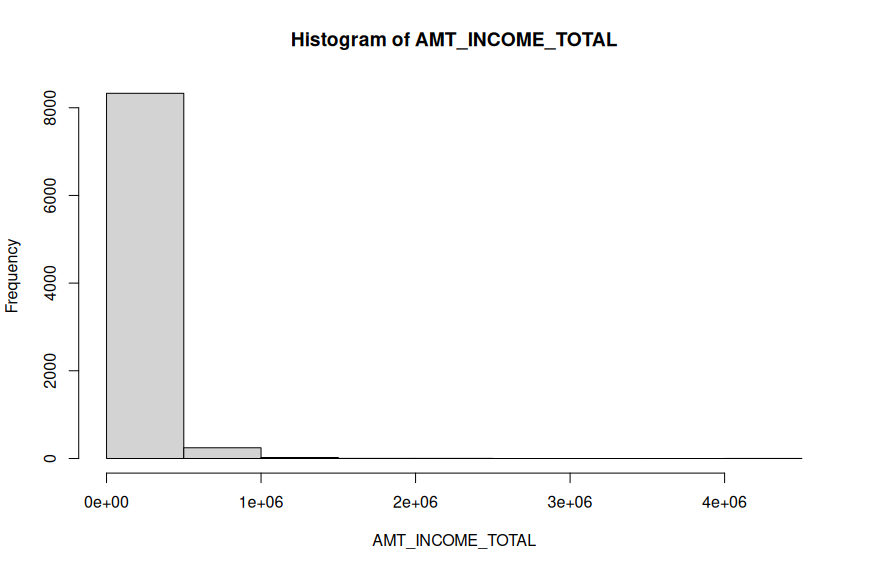
\includegraphics[width=0.45\textwidth]{img/83b37f62-d6f5-4e84-a7da-80b36e664b55.png}
  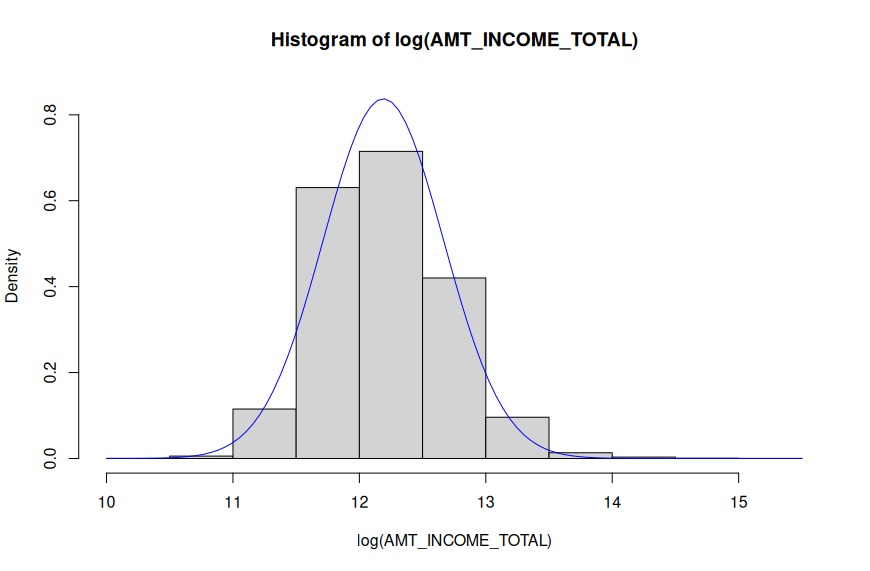
\includegraphics[width=0.45\textwidth]{img/c3b5fc12-a0e0-45e1-808b-eaa610e5e5ec.png}
\end{center}
\caption{Histogram of AMT\_INCOME\_TOTAL and $\log($AMT\_INCOME\_TOTAL$)$}
\end{figure}\\
Shifting our focus to the covariates, our initial examination involved assessing the correlation between our target variable (the logarithm of income) and the non-categorical covariates. The correlation coefficients range between $0.27$ and $-0.27$, with the most correlated variable being \\
\verb|REGION_POPULATION_RELATIVE_cubed|, which is the cubed transformation of a measure of population in the region of residence of the person. Turning to the categorical covariates, we first analyzed the relative frequency of each level in the categorical variable and then generated boxplots to visualize the relationships between these categorical covariates and the target variable, focusing on those we hypothesized to be better predictors of income.
\begin{figure}[h]
  \begin{center}  
  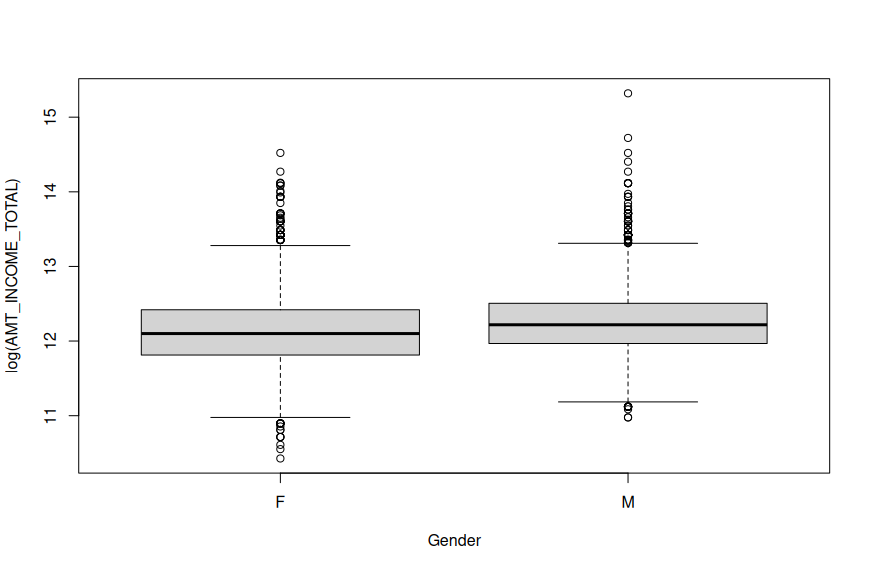
\includegraphics[width=0.32\textwidth]{img/392bcde4-d644-4740-8e7a-72728996638d.png}
  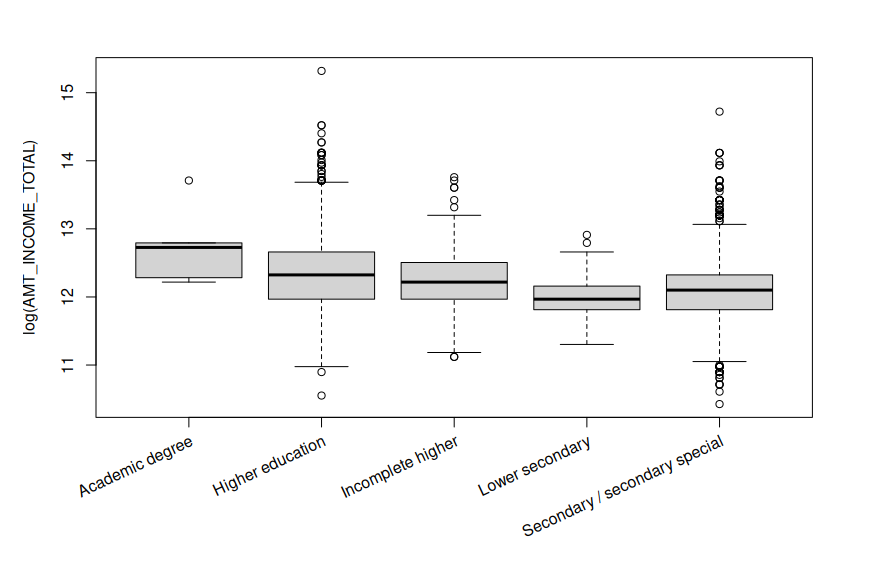
\includegraphics[width=0.32\textwidth]{img/3601fa4a-3df4-4656-831c-429f690699f2.png}
  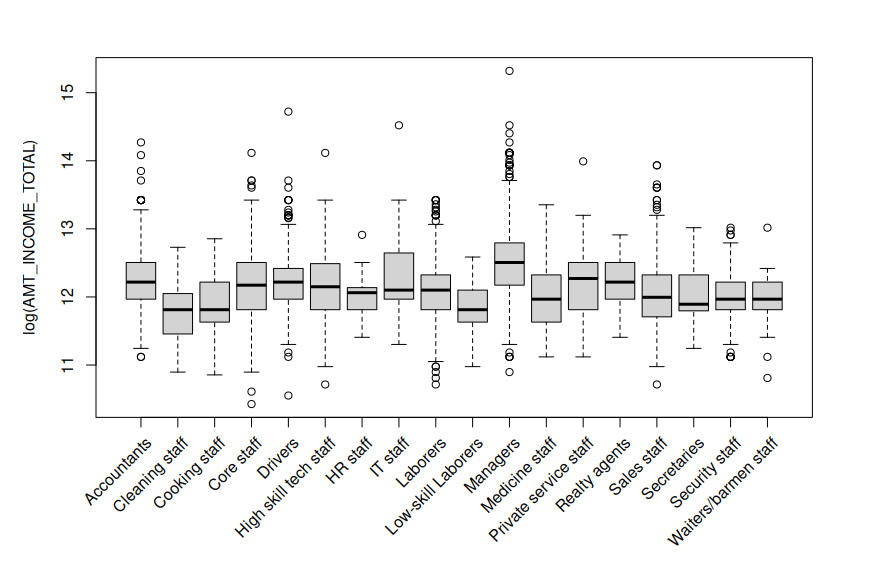
\includegraphics[width=0.32\textwidth]{img/8d368ccf-52dc-4c06-abaa-e6d8c64b5b73.png}
  \end{center}
\caption{Boxplots of $\log($AMT\_INCOME\_TOTAL$)$ with gender, education level, occupation}
\end{figure}
%\newpage
\section{Linear Regression}
In the upcoming section, our focus shifts to multivariate linear regression, aiming to construct a predictive model for our target variable using a subset of dataset features. We plan to employ three distinct model selection methods, evaluating their performance through k-fold cross-validation. This technique involves dividing the dataset into $k$ parts, using each as a validation set, and the union of the remaining $k-1$ parts as the training dataset. This allows us to reduce the risk of overfitting, a particularly pertinent concern given the abundance of features in our dataset. 

\subsection{Step-up model}
The first feature selection model we employ is the step-up/forward selection model, a form of stepwise regression model. Beginning with a parameter-free model, it tests each parameter individually. If no null hypotheses are rejected (p-value $> 0.05$), the model without parameters is chosen. Otherwise, the parameter with the smallest p-value is added, and the process is iteratively repeated until a suitable model is selected. While this method of model selection is quick to implement and often works well in finding small subsets of the covariates, it is worth mentioning that it has been criticized since the final model depends on the specific data used and thus may behave poorly out-of-sample. Since it strays from the scope of this paper, we link to a more in-depth discussion of this phenomenon \cite{Smith2018-uf}.\\
This method results in a linear model with $26$ features, achieving an $R^2$ of $0.3354$ and an adjusted $R^2$ of $0.3268$. The detailed feature list is available in the accompanying R file.

\subsection{Step-down model}
The step-down/backward elimination model, akin to step-up, is a form of stepwise regression. Unlike step-up, it starts with the full model and iteratively tests each parameter. If all null hypotheses are rejected, the entire model is chosen. Otherwise, the parameter with the largest p-value is removed, and the process is repeated. Given the similarities with the step-up method it also suffers from the same drawbacks we discussed above \cite{Smith2018-uf}. Importantly, results from the step-up and step-down methods may differ.\\
This method produces a linear model with 96 features, achieving an $R^2$ of $0.3495$ and an adjusted $R^2$ of $0.3357$.

\subsection{LASSO}
LASSO regression is another popular method for feature selection, it incorporates a penalty term on the absolute values of coefficients to promote sparsity. A crucial step in LASSO is selecting the optimal hyperparameter lambda, which controls the magnitude of the $l_1$ norm penalization. To determine the best lambda, the function \inlinecode{cv.glmnet()} is employed, automatically choosing the lambda associated with the minimum cross-validated mean squared error.\\
This method results in a linear model with $59$ features, achieving an $R^2$ of $0.3323$ and an adjusted $R^2$ of $0.3207$.

\subsection{Results}
As observed, all the $R^2$ values, both adjusted and regular, cluster between the values of $0.32$ and $0.34$, suggesting that roughly a third of the variance in monthly income can be explained by our models. This indicates that the relationship between the $\log(\verb|AMT_INCOME_TOTAL|)$ and our features is not very strong. Examining the F-tests for each different model, all of which are below 2.2e-16, confirms that each model is significantly better at predicting our target than the intercept.\\ 
Looking now at the residuals we assess if the assumptions of normality, homoscedacity and zero mean hold. In the step-up model (with the step-down model and LASSO being very similar), the mean residual is approximately -1.51e-17 (similar in magnitude for the other two models as well). However, both the Kolmogorov-Smirnov and Shapiro-Wilkins normality tests result in the rejection of normality for all methods and tests, potentially influenced by the ample sample size. Plotting the residuals against the target feature (illustrated here for the step-up method, with similar observations for the other methods) reveals a correlation coefficient of $0.815$ ($0.806$ and $0.819$ for the others), suggesting systematic underestimation of income for very high earners and overestimation for very low earners. We hypothesize missing predictors might be the cause of this. Despite this the homoscedastic assumption still seems to hold. 
\begin{figure}[h]
  \begin{center}
  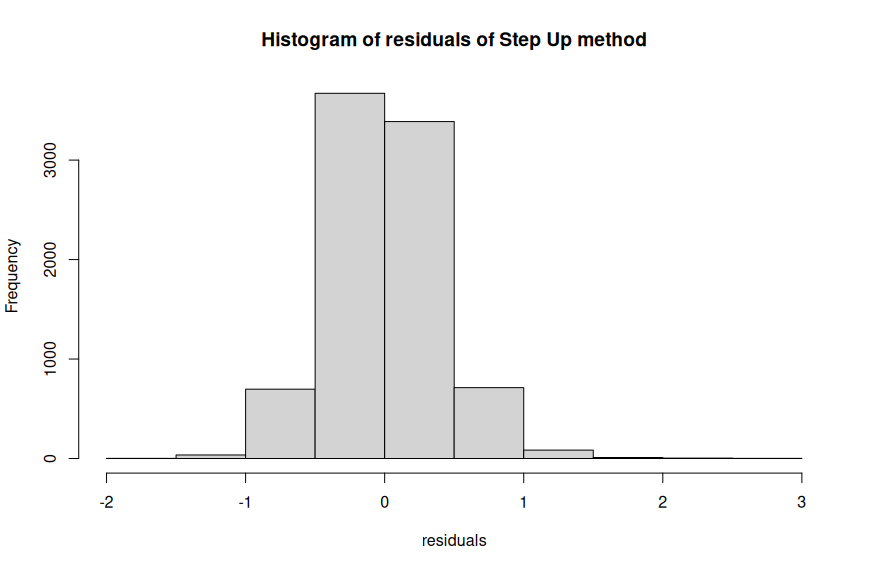
\includegraphics[width=0.32\textwidth]{img/20da428d-0af1-4f49-a7aa-66b7a1fe13bc.png}
  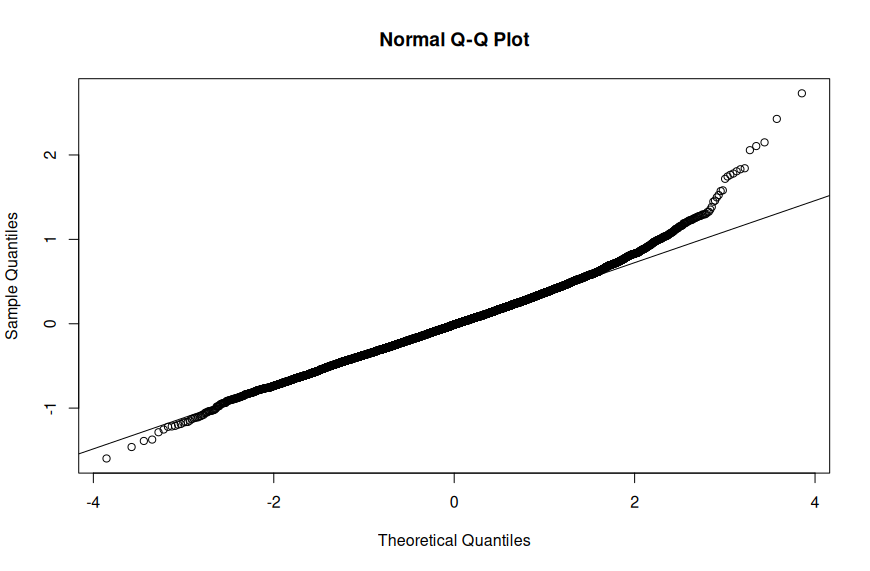
\includegraphics[width=0.32\textwidth]{img/6f01eecb-4039-4daa-ba0c-af7263bd658c.png}
  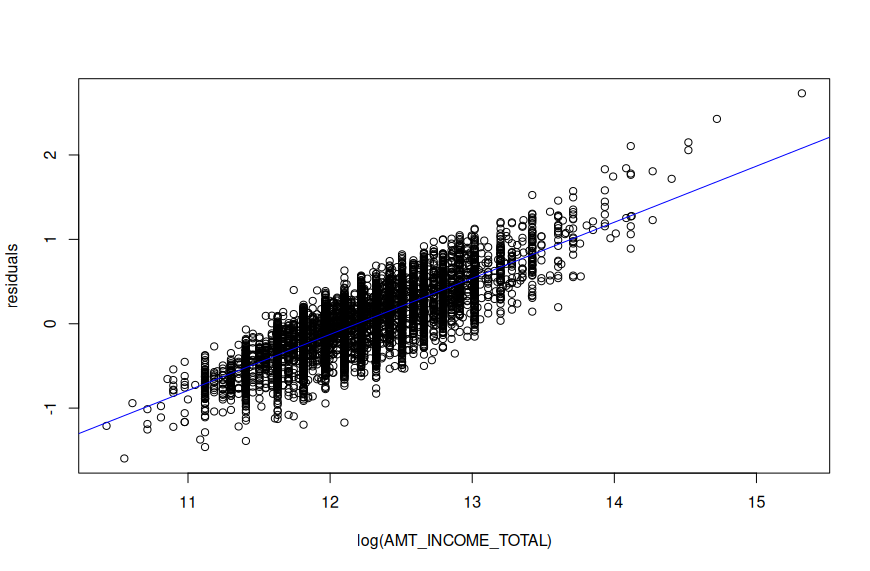
\includegraphics[width=0.32\textwidth]{img/b94b8a81-3824-47f5-a158-d8e9560e6ce2.png}
\end{center}
\caption{Histogram, qqplots and the plot of the residuals with line of best fit for the step-up model}
\end{figure}\\
Directing our attention to the Mean Squared Errors, we execute a for loop to calculate the MSE for each feature selection method as $k$ (referring to k-fold cross-validation) ranges from $2$ to $50$. The displayed MSE has been normalized by dividing it by the average of $\log(\verb|AMT_INCOME_TOTAL|)$, providing a standardized measure unaffected by the magnitude of the target variable. The average normalized MSE for the methods are: $0.02488$ for step-up, $0.02515$ for step-down, and $0.02479$ for LASSO. Although differences are marginal, it appears that the step-down model, with the most features, exhibits the worst performance in terms of MSE. This could indicate a potential case of data overfitting, as highlighted by cross-validation.
\begin{figure}[h]
  \begin{center}
  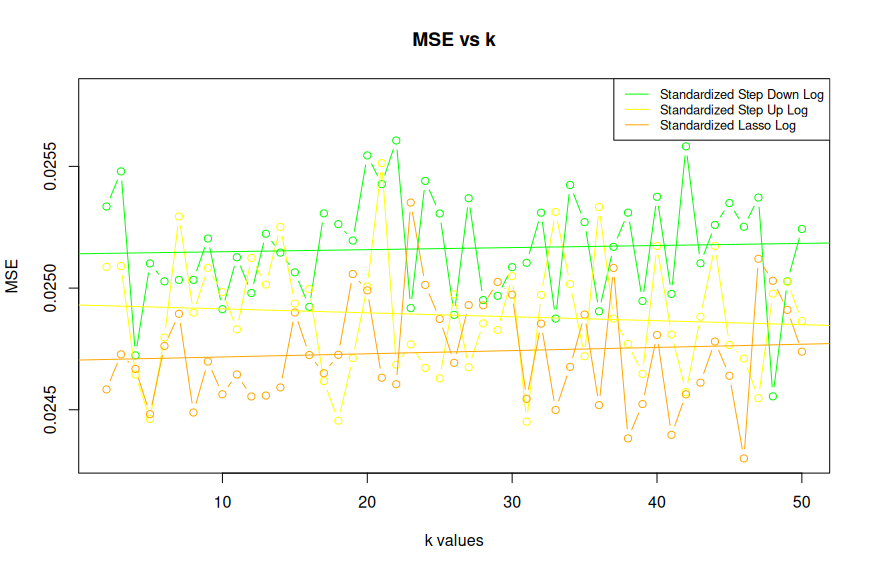
\includegraphics[width=0.32\textwidth]{img/4ce6b823-353d-4cd1-8960-77f9e7637f0c.png}
  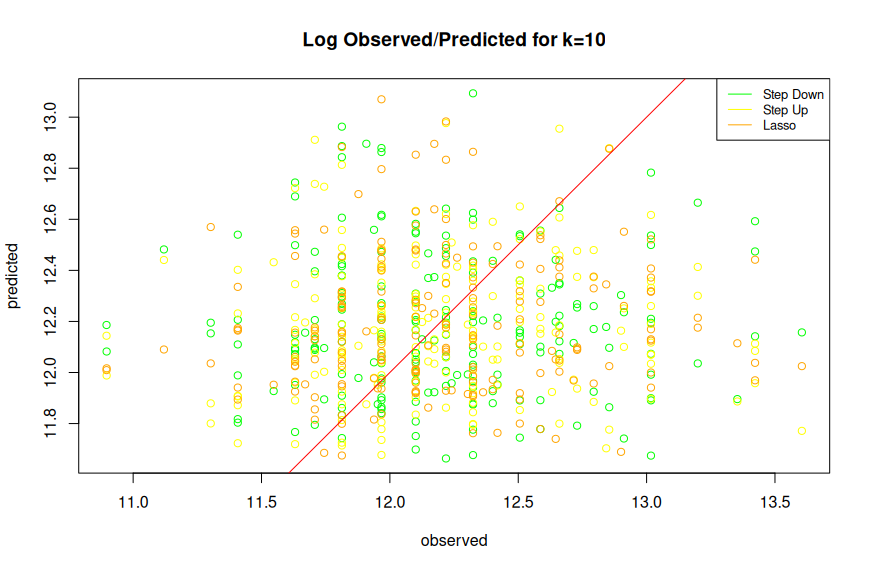
\includegraphics[width=0.32\textwidth]{img/5fbbbd32-5e14-434b-877f-548ddcf238b8.png}
  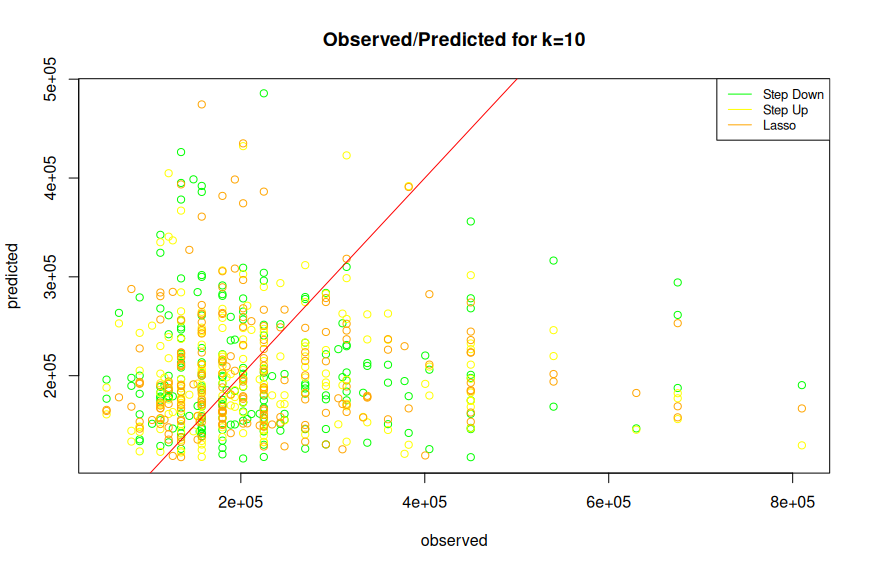
\includegraphics[width=0.32\textwidth]{img/d109caa8-4a84-490b-8da2-5df6a73cf0d6.png}
\end{center}
\end{figure}
\section{ANOVA of Gender and Job Type}
One further inquiry we wanted to investigate in this paper is the role is the role gender plays on the total income of a person; moreover, we also looked to see if this difference also depended on the type of job each person worked. To answer this question, we ran an ANOVA test using as features gender (\verb|CODE_GENDER|), occupation (\verb|OCCUPATION_TYPE|) and their interaction. Unlike the multivariate regression, we regressed on \verb|AMT_INCOME_TOTAL| directly. The primary outcomes of interest include the main effect for \verb|CODE_GENDER| (indicating meaningful income differences between males and females) and the interaction effect (revealing if this salary difference is consistent across occupations). The inexistence of a main effect of gender yields a p-value of 8.12e-25, signifying a systematic income difference between males and females. Additionally, the p-value for the interaction effect between gender and occupation is $0.00279$, strongly suggesting that this salary difference isn’t uniformly distributed across all occupations; instead, it is exacerbated in some while being reduced or even reversed in others.

\section{Conclusions, Limitations and Further Research}
In conclusion, we employed three models for predicting income based on diverse demographic and economic features, differing in their feature selection methods: step-up, step-down, and LASSO.\\
However, several limitations should be acknowledged. The dataset was not originally designed for this predictive purpose, introducing biases as it only reflects the income of individuals actively seeking a loan, potentially not representing the entire population. Additionally, bias arises from the handling of the \verb|OWN_CAR_AGE| variable, as removing missing data inadvertently narrows the focus to car owners, which may not be representative of the overall population. Subsequent analyses on this topic should address these issues.\\
Furthermore, the absence of features specifically collected for predicting the target variable implies the omission of potentially crucial predictors. Future research should consider incorporating geographical information, especially given the likely Russian origin of the data \cite{data-origin}, where income disparities between cities like St. Petersburg and Moscow and the rest of Russia are not currently accounted for and are only indirectly captured through features such as \verb|REGION_POPULATION_RELATIVE|.\\
A final crucial consideration involves the choice of using $\log(\verb|AMT_INCOME_TOTAL|)$ instead of\\ \verb|AMT_INCOME_TOTAL| as the target variable. Although done to address skewness, this decision may result in a loss of model interpretability. Further research could delve into a more comprehensive comparison of these two approaches, weighing the trade-offs between model performance and interpretability.
 \bibliography{bibliography} 
\end{document}
